\section{Introduction}
This project makes the drawings of different views of the building on the drawing sheets.

In this project, the user will be able to enter the specifications of the 
building through the web browser using Django (Python Web Framework) and 
on the back-end, the FreeCAD macros will use those input values to draw
the drawings of different views of the building on different drawing sheets. 
The output of the same can then be taken by a user in SVG, PDF and fcstd formats.
\subsection{Installation Guide}
To install Drawing FreeCAD project, you need to clone it from github.
\begin{itemize}
\item Go to terminal and type
\begin{lstlisting} 
git clone https://github.com/amrit3701/Drawing-FreeCAD.git
\end{lstlisting} 
\item Now go to the project directory by using
\begin{lstlisting} 
cd Drawing-FreeCAD
\end{lstlisting} 
\item Now running the below command.
\begin{lstlisting} 
python manange.py runserver
\end{lstlisting}
\item Now open $localhost:8000$ on the web-browser and you will see the below web page.
\begin{figure}[h!]
\begin{center}
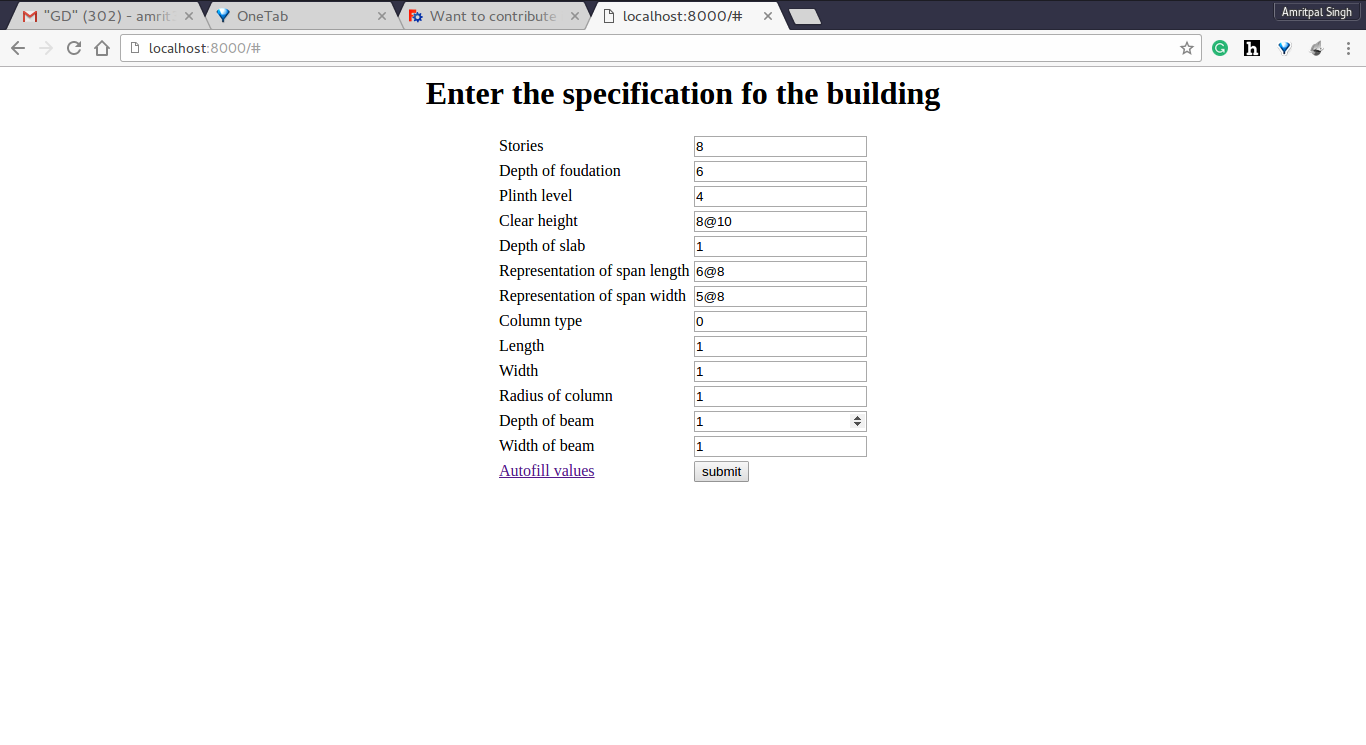
\includegraphics[scale=0.35]{images/first_page.png}
\caption{Front page}
\end{center}
\end{figure}
\end{itemize}

\section{FreeCAD workbenches used in this project}
\subsection{Part module}
The CAD capabilities of FreeCAD are based on the OpenCasCade kernel. The 
Part module allows FreeCAD to access and use the OpenCasCade objects and 
functions. OpenCascade is a professional-level CAD kernel, that features 
advanced 3D geometry manipulation and objects. The Part objects, unlike 
Mesh Module objects, are much more complex, and therefore permit much more 
advanced operations, like coherent boolean operations, modifications history 
and parametric behaviour.
\begin{figure}[h!]                                                       
\begin{center}                                                          
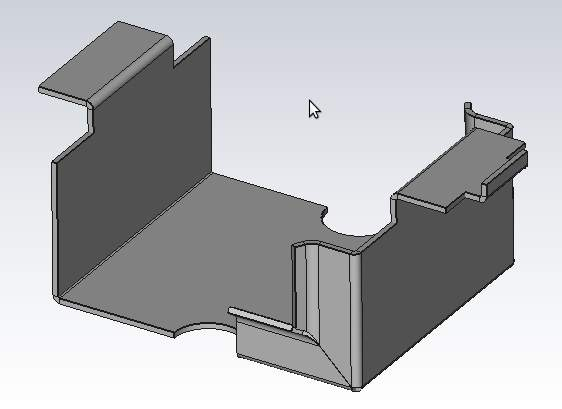
\includegraphics[scale=0.5]{images/Part_example.jpg}                     
\caption{Example of Part shapes in FreeCAD}                             \end{center} 
\end{figure}
\subsection{Draft module}
The Draft workbench allows to quickly draw simple 2D objects in the current 
document, and offers several tools to modify them afterwards. Some of these 
tools also work on all other FreeCAD objects, not only those created with 
the Draft workbench. It also provides a complete snapping system, and 
several utilities to manage objects and settings.
\subsection{Drawing module}
The Drawing module allows you to put your 3D work on paper. That is, to 
put views of your models in a 2D window and to insert that window in a drawing, 
for example a sheet with a border, a title and your logo and finally print that 
sheet. The Drawing module is currently under construction and more or less 
a technology preview!
\begin{figure}[h!]                                                       
\begin{center}                                                          
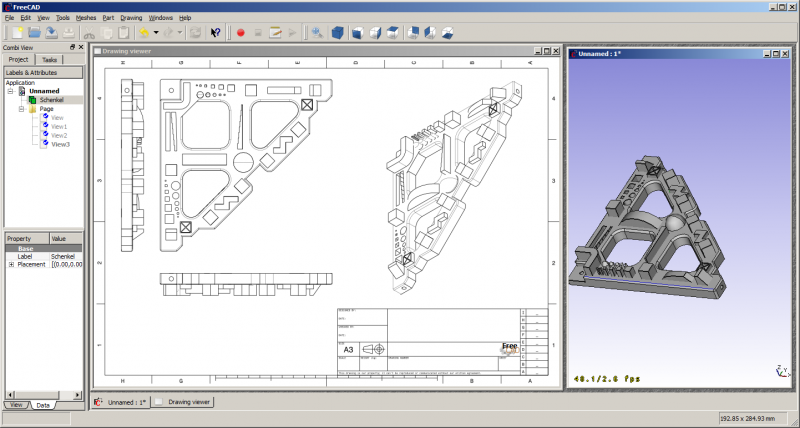
\includegraphics[scale=0.5]{images/Drawing_extraction.png}                     
\caption{Example of Drawing module in FreeCAD}                           \end{center}
\end{figure}

\section{Design implementation using Python scripting language}
Python is a programming language, very simple to use and very fast to learn. 
It is open-source, multi-platform, and can be used alone for a wide array of 
things, from programming simple shell scripts to very complex programs. But 
one of its most widespread uses is as a scripting language, since it is easy 
to embed in other applications. That's exactly how it is used inside FreeCAD. 
From the python console, or from your custom scripts, you can pilot FreeCAD, 
and make it perform very complex actions for which there is still no graphical 
user interface tool.\\
For example, from a python script, you can:
\begin{itemize}
\item create new objects
\item modify existing objects
\item modify the 3D representation of those objects
\item modify the FreeCAD interface
\end{itemize}
There are also several different ways to use python in FreeCAD:
\begin{itemize}
\item From the FreeCAD python interpreter, where you can issue simple commands like in a "command line"-style interface
\item From macros, which are a convenient way to quickly add a missing tool to the FreeCAD interface
\item From external scripts, which can be used to program much more complex things. like entire Workbenches.
\end{itemize}
\subsection{Writing python code}
There are two easy ways to write python code in FreeCAD: From the python 
console (available from the View -> Panels -> Python console menu) or from 
the Macro editor (Tools -> Macros). In the console, you write python commands 
one by one, which are executed when you press return, while the macros can 
contain a more complex script made of several lines, which is executed only 
when the macro is executed.
\begin{figure}[h!]                                                       
\begin{center}                                                          
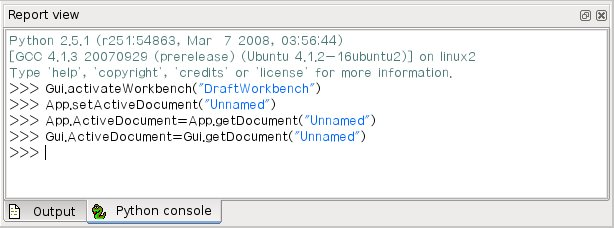
\includegraphics[scale=0.5]{images/Screenshot_pythoninterpreter.jpg}                     
\caption{Example of python scripting}
\end{center}
\end{figure} 

\section{Macros}
Macros are a convenient way to create complex actions in FreeCAD. You simply 
record actions as you do them, then save that under a name, and replay them 
whenever you want. Since macros are in reality a list of python commands, 
you can also edit them, and create very complex scripts.

In this project I have made many macros which are using for different purposes.
\begin{itemize}
\item \textbf{Builing macro:} This macro will create the model of building by
using the user input in 3D space of FreeCAD. For running this macro in the 
project I have used the below command.
\begin{lstlisting}
freecadcmd builing_macro.py
\end{lstlisting}
\begin{figure}[h!]                                                      
\begin{center}                                                          
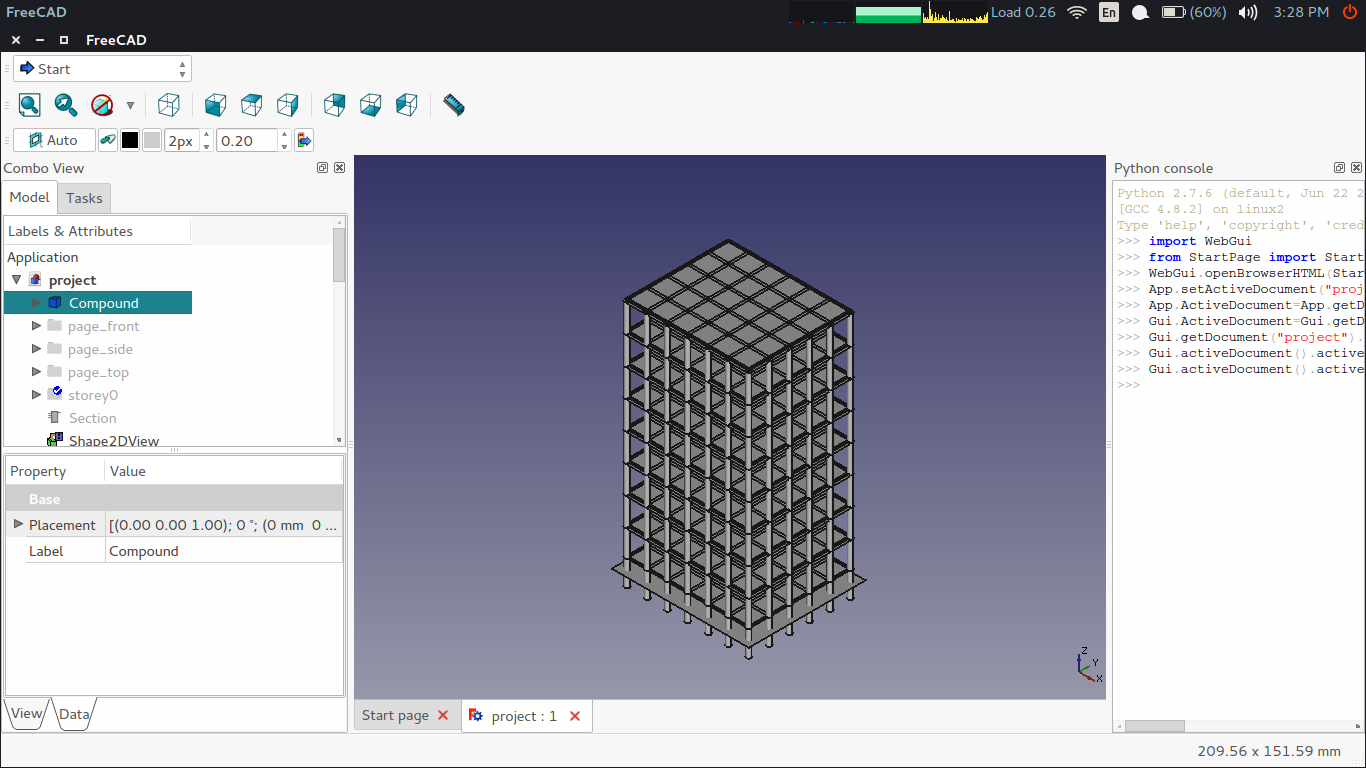
\includegraphics[scale=0.35]{images/building_macro.png}
\caption{Example of building macro}                                   
\end{center}                                                            
\end{figure}
\item \textbf{Drawing macro:} This macro will draw the drawing of different 
views (top, front and side view) of the builing along with sectional view of each 
building storey on the drawing sheet.
(3D model).
\begin{lstlisting}                                                      
freecadcmd drawing.py                                                
\end{lstlisting}
\begin{figure}[h!]                                                      
\begin{center}                                                          
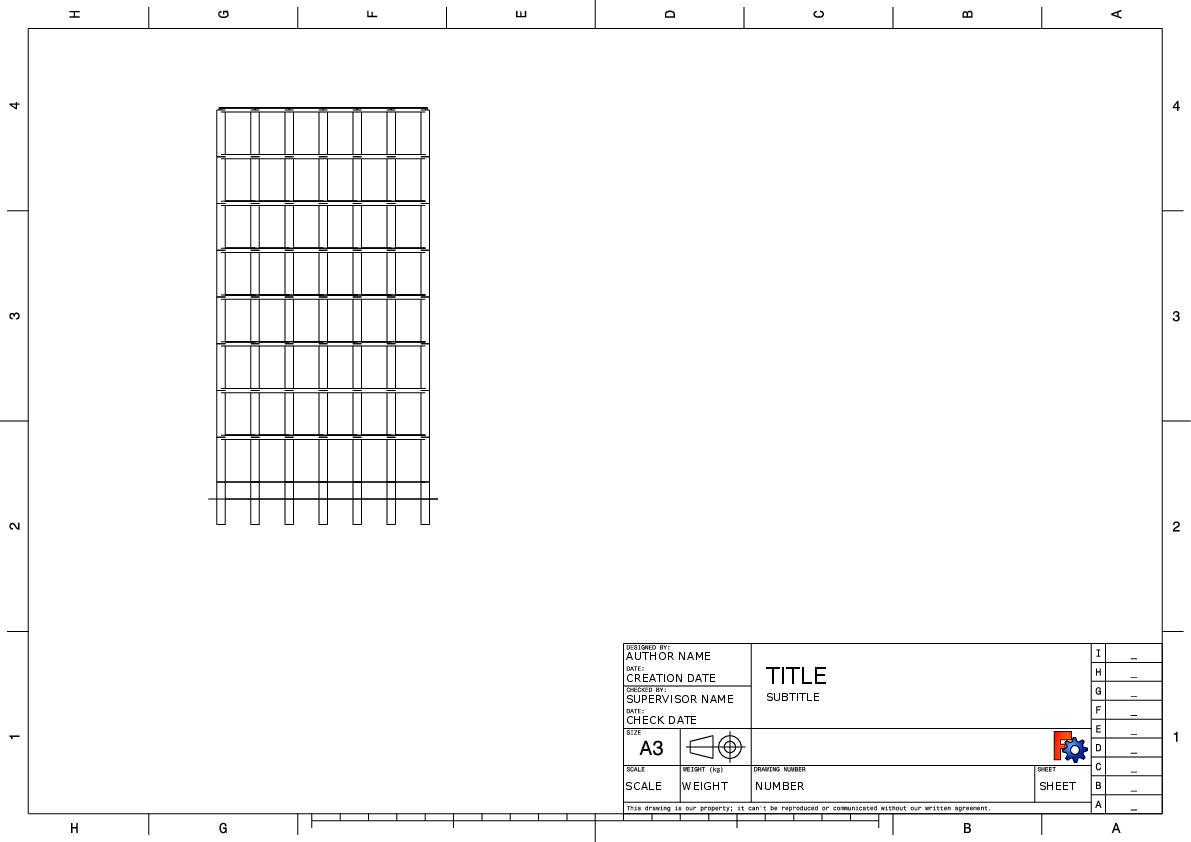
\includegraphics[scale=0.35]{images/page_side.png}
\caption{Example of drawing macro}                                   
\end{center}                                                            
\end{figure}
 
\item \textbf{Saving drawing macro:} This macro will save the drawing of the 
building in SVG (Scalable Vector Graphics) and then convert SVG file into PDF 
(Portable Document Format).
\begin{lstlisting}                                                      
freecadcmd save_drawing.py                                                
\end{lstlisting} 
\end{itemize}
